\documentclass[../main.tex]{subfiles}
\begin{document}

\section{Introduzione}

In questo capitolo verranno presentate le proposte sperimentali sviluppate per indagare le capacità dei modelli di VQA nel contesto medico del \textit{KvasirVQA}. 

A partire dalle tecniche e dai modelli analizzati nei capitoli precedenti, sono state definite strategie sperimentali volte a testare l'efficacia di diverse architetture e approcci, includendo sia modelli basati su tecniche tradizionali, sia soluzioni più recenti che sfruttano il prompting, il \textit{Chain-of-Thought} e i transformers. 
L'obiettivo principale è quello di esplorare le potenzialità dei modelli multimodali nell'elaborazione di immagini diagnostiche e domande strutturate, valutandone i limiti e le possibili aree di miglioramento.

Le proposte sperimentali includono:
\begin{itemize}
    \item L'applicazione di tecniche di prompting, con particolare attenzione al \textit{templating} e al \textit{Chain-of-Thought}.
    \item Adozione di architetture personalizzate per verificare l'efficacia sui dati a disposizione.
    \item Variazioni procedurali per affrontare il task in forma di classificazione multilabel, oltre che multiclasse.
    \item Utilizzo di un'architettura moderna e basata su transformers, addestrata per adattarsi al contesto del KvasirVQA.
\end{itemize}

L'obiettivo di queste proposte è non solo di testare l'efficacia di tecniche avanzate, ma anche di fornire insight utili per l'ottimizzazione dei modelli di VQA in ambito medico, contribuendo così a colmare le lacune identificate nella ricerca attuale.
I risultati ottenuti verranno discussi nel capitolo successivo, con un'analisi dettagliata delle prestazioni e del confronto tra le diverse configurazioni sperimentali.

\section{Classificazione multilabel}

La scelta di trasformare il task di classificazione multiclasse in classificazione multilabel nasce dall'analisi delle peculiarità del dataset KvasirVQA e delle caratteristiche intrinseche del task di VQA. 
Questa sezione illustra le motivazioni che hanno portato a questa decisione, i vantaggi attesi e le modifiche necessarie per implementare tale approccio.

Nel task di classificazione multiclasse, ogni combinazione di opzioni rappresenta una risposta unica e distinta. Tuttavia, questo approccio presenta delle limitazioni significative nel contesto del KvasirVQA:

\begin{itemize}
    \item \textbf{Elevato numero di classi:} Il dataset presenta 469 risposte uniche generate da combinazioni di opzioni, aumentando significativamente la complessità del task e il rischio di \textit{under-fitting}, specialmente con dataset di dimensioni limitate come quello con cui stiamo lavorando.
    \item \textbf{Relazioni tra le risposte:} Le risposte non sono sempre mutuamente esclusive. Ad esempio, alcune domande ammettono combinazioni di opzioni come risposte valide (ad esempio, presenza simultanea di più anomalie), rendendo più naturale il trattamento del problema come task multilabel.
    \item \textbf{Generalizzazione:} Un task multilabel permette al modello di apprendere in modo più flessibile, associando ogni opzione a un'etichetta binaria indipendente. Questo approccio facilita la generalizzazione a combinazioni non viste durante l'addestramento.
\end{itemize}

La trasformazione in classificazione multilabel consente di rappresentare ciascuna risposta come un vettore di etichette binarie, dove ogni posizione del vettore indica la presenza (1) o l'assenza (0) di una particolare opzione.

\subsection{Vantaggi del task multilabel}

Il passaggio a un task multilabel offre numerosi vantaggi pratici e metodologici:
\begin{itemize}
    \item \textbf{Riduzione della complessità:} Trattando ogni opzione come etichetta indipendente, il modello si concentra sull'identificazione di caratteristiche specifiche, riducendo la complessità computazionale rispetto alla gestione di un numero elevato di classi distinte.
    \item \textbf{Flessibilità nelle risposte:} Il modello è in grado di prevedere combinazioni di opzioni non presenti nel set di addestramento, migliorando la capacità di adattarsi a nuovi scenari.
    \item \textbf{Mitigazione dello sbilanciamento:} La rappresentazione multilabel consente di bilanciare il peso delle opzioni meno rappresentate senza dover intervenire direttamente sulla distribuzione delle risposte complete.
    \item \textbf{Adattabilità a modelli generativi:} Questo approccio è concettualmente allineato a tecniche basate su modelli generativi e \textit{templating}, che formulano le risposte come insiemi di opzioni selezionate.
\end{itemize}

\subsection{Implementazione tecnica}

Per implementare il task multilabel, sono state apportate le seguenti modifiche alla pipeline di addestramento:
\begin{itemize}
    \item \textbf{Rappresentazione delle risposte:} Ogni risposta è stata trasformata in un vettore binario di lunghezza pari al numero di opzioni uniche (58). Ad esempio, una risposta contenente due opzioni sarebbe rappresentata come un vettore con due valori pari a 1 e i restanti pari a 0.
    \item \textbf{Funzione di perdita:} La \textit{Binary Cross Entropy Loss} è stata adottata al posto della \textit{Cross Entropy Loss}, per calcolare la perdita indipendentemente per ciascuna etichetta.
    \item \textbf{Modifica dell'output del modello:} Lo strato finale del modello è stato adattato per produrre logits per ciascuna delle 58 etichette, seguite da una funzione \textit{sigmoid} per ottenere probabilità indipendenti.
\end{itemize}

Nonostante i vantaggi, l'approccio multilabel presenta alcune sfide:
\begin{itemize}
    \item \textbf{Interpretazione delle soglie:} La scelta di una soglia per determinare la presenza di un'etichetta è cruciale e può influire significativamente sulle prestazioni del modello. Nelle implementazioni per questa tesi, la soglia è stata impostata a 0,5.
    \item \textbf{Dipendenza dai dati:} Il task multilabel richiede un dataset ben bilanciato per evitare che il modello ignori le etichette meno rappresentate.
    \item \textbf{Aumento delle risorse computazionali:} Sebbene il numero di classi sia ridotto, la necessità di calcolare probabilità per ciascuna etichetta può aumentare il costo computazionale.
\end{itemize}

\section{Fine-tuning del modello ViLT sul dataset KvasirVQA}

Il modello ViLT è stato scelto per il fine-tuning grazie alla sua architettura leggera e alla capacità di elaborare simultaneamente immagini e testo utilizzando un unico Transformer. A differenza di altri modelli multimodali che si basano su un backbone visivo separato, ViLT integra direttamente i token visivi e testuali in uno spazio comune, risultando più efficiente in termini di calcolo e memoria.
Sono stati quindi eseguiti degli addestramenti e poi dei test per verificare la capacità del modello di performare nel contesto.

\subsection{Preparazione dei dati}

\subsubsection{Elaborazione delle immagini}

Le immagini del dataset KvasirVQA sono state preprocessate utilizzando il \textit{ViLTProcessor} fornito dalla libreria \textit{HuggingFace}. Questo strumento automatizza operazioni fondamentali come il ridimensionamento delle immagini, il padding e la normalizzazione dei pixel, garantendo una rappresentazione coerente degli input visivi.

In particolare, il metodo \textit{pad} del \textit{ViLTProcessor} è stato utilizzato per creare un padding uniforme, adattandole alle dimensioni della larghezza e altezza maggiori presenti nel batch e preservando le proporzioni originali dell'immagine. 
Questa operazione ha evitato distorsioni che avrebbero potuto compromettere l'accuratezza delle previsioni del modello.

\begin{figure}[H]
    \centering
    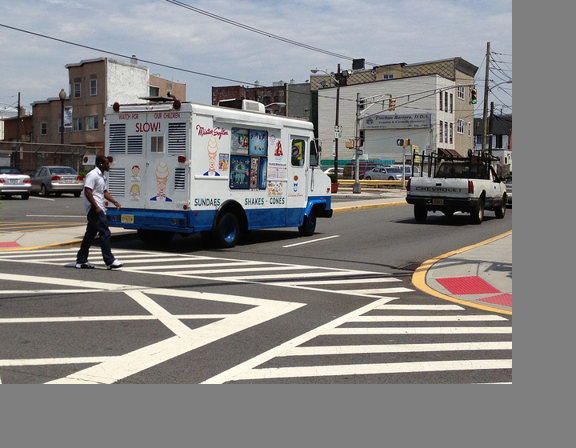
\includegraphics[width=0.5\linewidth]{static/vilt_padding.png}
    \caption{Esempio di immagine con padding aggiunto dal ViLTProcessor}
    \label{fig:enter-label}
\end{figure}

\subsubsection{Elaborazione del testo}

Le domande e risposte del dataset sono state tokenizzate utilizzando il tokenizer associato al Transformer di ViLT. 
Analizzando il vocabolario a disposizione del tokenizer del modello ViLT base scelto, sono state rilevate 22 parole non presenti, che sono state aggiunte prima dell'addestramento.

Nel dettaglio, i vocaboli che \textbf{non} erano presenti precedentemente sono i seguenti: 

\begin{quote}
    gastroscopy / artefact / snare / barretts / colonoscopy / forceps / endoscopy / 20mm / polyp / ulcerative / pylorus / iia / ileum / 10mm / hemorrhoids / abnormality / biopsy / oesophagitis / colitis / 5mm / polyps / cecum
\end{quote}

\subsection{Configurazione del modello}

Per il fine-tuning, è stato utilizzato il checkpoint pre-addestrato \textit{"dandelin/vilt-b32-mlm"} disponibile su \textit{HuggingFace}.
L'architettura di ViLT è stata modificata per adattarla al task specifico del KvasirVQA nel seguente modo:
\begin{itemize}
    \item Lo strato finale \textit{fully connected} è stato rimodulato per produrre output corrispondenti al numero di risposte uniche nel dataset.
    \item Per il task di classificazione multiclasse, è stata utilizzata una funzione \textit{Softmax} per trasformare i logits in una distribuzione di probabilità.
    \item Per il task multilabel, è stata adottata una funzione \textit{sigmoid}, permettendo al modello di generare probabilità indipendenti per ciascuna etichetta.
\end{itemize}

\subsection{Configurazione dell'addestramento}

\subsubsection{Iperparametri}

Prima di procedere a elencare la configurazione scelta per l'addestramento, precisiamo che per il \textit{learning rate} sono stati scelti valori volutamente molto bassi dal momento che la \textit{backbone} del modello è rimasta intatta e soltanto la testa è stata riaddestrata per specializzarsi, permettendo quindi una maggiore stabilità in fase di addestramento e minori oscillazioni nella minimizzazione della funzione di perdita.

L'addestramento è stato configurato con i seguenti iperparametri, scelti tramite una serie di esperimenti preliminari:

\begin{itemize}
    \item Learning rate: 4e-5
    \item Batch size: 16.
    \item Numero di epoche: 200.
    \item Ottimizzatore: AdamW.
    \item Scheduler: ReduceLROnPlateau.
    \item Pazienza: 5
    \item Min. Delta: 0.001
    \item Epoche Minime: 5
\end{itemize}

Questa scelta di iperparametri è risultata valida per entrambi gli approcci al problema, sia multiclasse che multilabel. 
Tuttavia, riteniamo che il fattore d'influenza principale dietro i risultati sia da attribuire ai dati in sé e alle criticità già menzionate nel capitolo relativo al KvasirVQA.

\subsubsection{Loss function}

Per il task multiclasse, è stata utilizzata la \textit{Cross Entropy Loss}, mentre per il task multilabel è stata adottata la \textit{Binary Cross Entropy Loss}.

\subsubsection{Early Stop}

Per evitare l'overfitting, è stato applicato un meccanismo di \textit{early stop} che prevede una soglia di tolleranza, un delta e un minimo di epoche, in modo da interrompere l'addestramento in caso di mancati miglioramenti ripetuti, ma garantendo comunque un minimo di epoche prima dell'attivazione del meccanismo.

\begin{lstlisting}
class EarlyStopper: 
    def __init__(self, patience=1, min_delta=0, min_epochs=0):
        self.min_epochs = min_epochs
        self.patience = patience
        self.min_delta = min_delta
        self.counter = 0
        self.epoch_counter = 0
        self.min_validation_loss = float('inf')
        
    def early_stop(self, validation_loss):
        self.epoch_counter += 1
        
        if self.epoch_counter < self.min_epochs:
            return False
        
        if validation_loss < self.min_validation_loss:
            self.min_validation_loss = validation_loss
            self.counter = 0
        elif validation_loss >= (self.min_validation_loss + self.min_delta):
            self.counter += 1
            if self.counter >= self.patience:
                return True
        return False
\end{lstlisting}

\subsubsection{Scheduler}

Oltre all'utilizzo del meccanismo di early stop per la regolarizzazione, sono stati testati vari \textit{scheduler} per la gestione del learning rate, messi a disposizione da \textit{PyTorch}. 
Quello che è risultato essere più valido dai test effettuati è stato lo scheduler \textit{ReduceLROnPlateau}, per la riduzione del learning rate nelle fasi di stallo dell'addestramento.

\section{Architettura custom}

L’obiettivo dietro la proposta di un'architettura personalizzata è analizzare come un modello costruito su misura possa affrontare le peculiarità del dataset, in particolare le domande che combinano componenti testuali e visive complesse. 
In particolare è stata pensata un'architettura ispirata ai metodi tradizionali di fusione multimediale dei \textit{joint-embeddings} della componente testuale e visiva, distinguendo poi il task in classificazione multiclasse della risposta o multilabel, per verificare l'efficienza dei due diversi metodi. 
Prendendo come punto di partenza l'architettura pensata in \cite{DBLP:journals/corr/AndersonHBTJGZ17}, ne è stata pensata una versione che potesse adattarsi e affrontare le peculiarità del KvasirVQA, quali scarsezza di dati e di annotazioni precise per le immagini.

\subsection{Architettura}

L’architettura custom proposta si basa su una combinazione di un estrattore di caratteristiche visive e un modulo di elaborazione testuale, integrati tramite una fase di fusione multimodale. Gli elementi principali dell'architettura sono un estrattore di caratteristiche visive (\textit{feature extractor}) e un modulo per l'elaborazione testuale.

\begin{figure}[H]
    \centering
    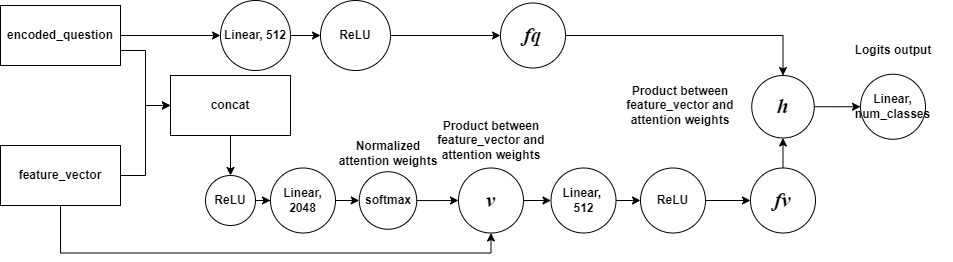
\includegraphics[width=1.05\linewidth]{static/CustomNN.drawio.png}
    \caption{Schema riassuntivo dell'architettura completa}
    \label{fig:enter-label}
\end{figure}

\subsubsection{Estrattore di Caratteristiche Visive}

Per la scelta dell'estrattore visivo, sono stati testati diversi modelli pre-addestrandoli nel riconoscimento delle immagini di dataset originali \textit{HyperKvasir} e \textit{Kvasir Instrument}, scegliendo infine quello con la percentuale di accuracy più alta in base all'F1 macro score.
Il migliore tra questi modelli, ovvero una rete \textit{ResNet50}, è stato utilizzato quindi come backbone per l'estrazione delle features visive globali dall'immagine.

\subsubsection{Modulo di Elaborazione Testuale}

Per la codifica delle domande, è stato utilizzato un modello \textit{BERT-like} \cite{alsentzer2019publiclyavailableclinicalbert}, specializzato in ambito medico e quindi ritenuto adatto al compito da affrontare. 
Le sequenze di parole vengono quindi tokenizzate e trasformate in embedding per ottenere una rappresentazione contestualizzata delle domande.

I token non presenti tra quelli conosciuti sono stati aggiunti, e sono i seguenti: 

\begin{quote}
    polyp / barretts / polyps / oesophagitis / 10mm / cecum / ip / colitis / abnormality / abnormalities / forceps / anatomical / gastroscopy / biopsy / colonoscopy / ileum / 5mm / hemorrhoids / endoscopy / 20mm / ulcerative / paris / artefact / pylorus / iia / snare
\end{quote} 

\subsubsection{Attenzione normalizzata}

Nel tentativo di replicare un meccanismo di attenzione funzionante e che sfruttasse gli input sia visivi che testuali, è stato integrato l'utilizzo dell'attenzione normalizzata nel seguente modo: 

Concatenando il vettore ottenuto dalla ResNet \textit{v} di dimensione 2048 insieme alla codifica del testo \textit{q} di dimensioni 768.
Il vettore risultante $\alpha$ viene quindi riproiettato per avere una dimensione uguale a \textit{V}, normalizzato utilizzando una funzione softmax e infine viene calcolato il prodotto tra $\alpha$ e \textit{v}.

\subsubsection{Fusione Multimodale}

Dopo aver applicato il meccanismo di attenzione normalizzato su \textit{v}, è possibile infine procedere alla fusione multimodale di caratteristiche visive e testuali.
Facciamo dunque passare \textit{q} e  \textit{v} entrambi separatamente per layer non lineari e lineari per riproiettarli con dimensioni uguali, moltiplichiamoli e usiamo l'output come input per l'ultimo layer di classificazione.

\subsubsection{Strato Finale di Classificazione}

L'ultimo layer che si occupa della classificazione è un layer lineare di dimensione variabile in base al task multiclasse o multilabel, con dimensione pari al numero di classi nel dataset. 
In ogni caso, l'utilizzo è quello di effettuare classificazione sulle logits, variando la funzione di attivazione in uscita:

Per il task multilabel, è stata utilizzata una funzione di attivazione \textit{sigmoid}, mentre per il task multiclasse si è utilizzata una funzione \textit{softmax}.

\subsection{Configurazione dell’Addestramento}

Il modello è stato addestrato utilizzando \textbf{PyTorch}, con i seguenti parametri principali:

\begin{itemize}
    \item Learning rate: 4e-4
    \item Batch size: 32
    \item Numero di epoche: 200.
    \item Ottimizzatore: AdamW.
    \item Scheduler: ReduceLROnPlateau.
    \item Pazienza: 5
    \item Min. Delta: 0.001
    \item Epoche Minime: 5
\end{itemize}

\subsection{Visualizzazione componente visiva}

Per una comprensione migliore del funzionamento delle architetture custom, è stato utilizzato l'algoritmo Grad-CAM per generare le heatmap e visualizzare le attivazioni del modello. 
In particolare, sono state generate le immagini ottenute dal feature extractor già menzionato.
Alcuni esempi saranno presentati insieme agli esperimenti nel prossimo capitolo, generati grazie alla libreria PyTorch dedicata \cite{jacobgilpytorchcam}.

\section{Prompting applicato al KvasirVQA}

In questa sezione verranno descritti gli approcci basati sul prompting utilizzati per esplorare le prestazioni di diversi modelli multimodali sul dataset KvasirVQA. Sono state applicate due tecniche principali di prompting, \textit{templating} e CoT, al fine di migliorare la comprensione testuale e il ragionamento visivo-linguistico dei modelli. 
Le tecniche di prompting applicate sono state studiate per tentare innanzitutto di guidare i modelli nella generazione di una risposta coerente con il contesto, cercando di instradarli tramite presentazione di opzioni per la risposta o tramite l'esplicitazione del ragionamento fatto per arrivare a una soluzione.

\subsection{Modelli Utilizzati}

Le tecniche di prompting sono state testate su una selezione di modelli multimodali descritti nel capitolo sullo stato dell'arte:

\begin{itemize}
    \item BLIP
    \item GIT
    \item LLaVA
\end{itemize}

\subsection{Templating}

Il \textit{templating} è stato applicato utilizzando una serie di schemi predefiniti per standardizzare l’interazione tra input testuali e modelli. Questa tecnica mira a fornire al modello una struttura coerente per comprendere il task e generare risposte.

\subsubsection{Template Utilizzati}

Di seguito alcuni esempi di template adottati:
\begin{lstlisting}
Template-1:

You are given the following question:
Question: <q>
Below are the possible options:
Options: <o>
Respond using only the options provided. If multiple options apply, separate them with a semicolon (';').

Template-2:

Based on the following question:  
Question: <q>  
Choose the most appropriate answer(s) from the provided options:  
Options: <o>  
Please respond using one or more of the options, separated by a semicolon (';'), if applicable.  
Answer:  

\end{lstlisting}

\subsection{Chain-of-Thought (CoT)}

La tecnica \textit{Chain-of-Thought} è stata impiegata per stimolare il ragionamento passo-passo dei modelli. Questa tecnica guida il modello a suddividere il problema in passaggi logici prima di fornire una risposta.

\subsubsection{Prompt per il Chain-of-Thought}

I prompt per il CoT sono stati progettati per incoraggiare i modelli a esplicitare il ragionamento. Alcuni esempi includono:

\begin{lstlisting}

CoT-1:

Q: <q>
Options: <o>
A: Let's think step-by-step.  

CoT-2:

Q: <q>  
Options: <o>  
A: Let's think step-by-step.  
1. First, identify the key information in the question.  
2. Next, relate this information to the available options.  
3. Eliminate any options that do not align with the question.  
4. Finally, based on the analysis, respond with the most appropriate option(s), separated by a semicolon (';') if multiple answers apply.  
Answer: 

\end{lstlisting}

I risultati dettagliati delle tecniche di prompting applicate ai modelli elencati verranno discussi nel capitolo dedicato agli esperimenti, con analisi comparative e approfondimenti sull'efficacia delle diverse configurazioni.

\end{document}